\documentclass[10pt]{article}
\usepackage[margin=2.5cm]{geometry}
\usepackage[T1]{fontenc}
\usepackage{lmodern}
\usepackage{enumitem}
\usepackage{tikz}
\usetikzlibrary{arrows.meta,calc}
\usepackage[hidelinks]{hyperref}
\setlist{itemsep=2pt,topsep=4pt}

\title{Zero human in the inner loop}
\author{Position note on why Pathfinder exists}
\date{25 October 2026}

\begin{document}
\maketitle

\section{Implications of LMs' current cognitive performance}

\textbf{(A1)} language models will soon match humans at solving and checking
most scientific and technical tasks; x10 cheaper and x10 faster. A possible
x100 increase in the rate of knowledge unit production. 

[not accounting
for the training costs; just assume you have LMs vs expert humans]

Arguably, this is already the case in mathematics (Navier-Stokes). 

The purpose of this note is to explore the likely consequences of this cognitive
emergence in the tech and science progress.

We consider a simple cyclic model of tech and science progress. 

Hereafter the ``inner loop''.

\begin{center}
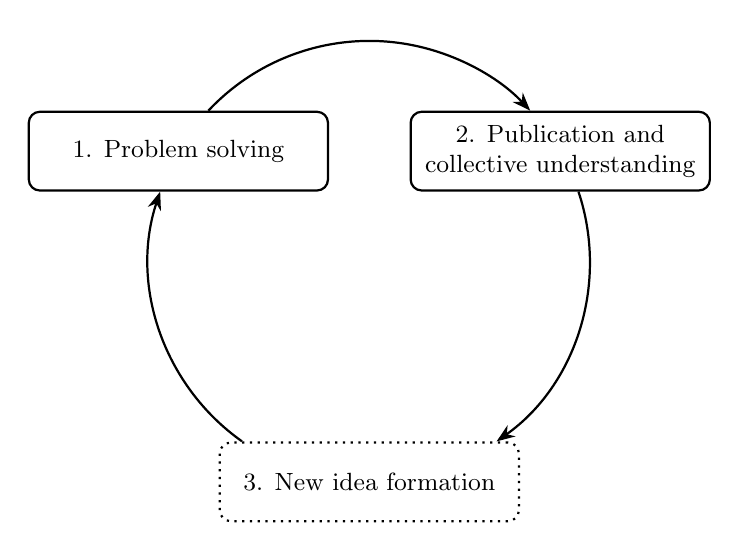
\begin{tikzpicture}[
  stage/.style={draw, rounded corners, align=center, minimum width=3.8cm,
    minimum height=1cm, font=\small},
  >={Stealth}, thick
]
  \node[stage] (solving) at (150:2.8cm) {1. Problem solving};
  \node[stage] (publication) at (30:2.8cm) {2. Publication and\\collective understanding};
  \node[stage, dotted] (ideas) at (270:2.8cm) {3. New idea formation};
  % Centers are 120 degrees apart; all arrows follow their circumcircle.
  % Trim each circular arc at its intersection with the box border.
  \draw[->] let \p1=(solving.north), \p2=(publication.north) in
    ({180-asin(\y1/2.8cm)}:2.8cm)
    arc[start angle={180-asin(\y1/2.8cm)},
        end angle={asin(\y2/2.8cm)}, radius=2.8cm];
  \draw[->] let \p1=(publication.south), \p2=(ideas.north) in
    ({asin(\y1/2.8cm)}:2.8cm)
    arc[start angle={asin(\y1/2.8cm)},
        end angle={asin(\y2/2.8cm)}, radius=2.8cm];
  \draw[->] let \p1=(ideas.north), \p2=(solving.south) in
    ({180-asin(\y1/2.8cm)}:2.8cm)
    arc[start angle={180-asin(\y1/2.8cm)},
        end angle={180-asin(\y2/2.8cm)}, radius=2.8cm];
\end{tikzpicture}
\end{center}



\section{Conditions for the cycle to speed-up}
It follows that -to the extent rate of knowledge production is the goal to
maximise (as opposed eg to being a museum of pre-AI cognition
capabilities)- the planner ought to replace human math-solving with AI math solving in
math departments.

However, the cycle also needs idea formation. It is not enough to solve quickly and efficiently,
one has to replenish the idea tank. At the same speed. Or else no speed up of the cycle.

Focus shifts from problem solving (step 1) to idea generation (step 3 and whatever
replaces step 2 for LMs. \textbf{(A2)} Which we assume is trivial (ie LMs read and ingest fast).
The
scarce resource in research is no longer to solve problems but to formulate
good ones. 

\textbf{(A3)} Step 2 is human understanding (T. Tao digestion process) or
collective and continuous learnig process. For an LM it would be
training/learning.\footnote{LMs don't locate knowledge so much as
reconstruct it; maths is most re-constructible knowledge system, since
there is nothing to measure} It is valuable because it leads to new ideas.
[publication system is way to gatekeep for orginality and guarantee novelty
(correctness too)]

It is often said these days that humans cannot understand new math results
at the speed agents produce them.   If human understanding is a necessary ingredient of the inner loop,
then AI will not accelerate science. Because humans cannot produce new
ideas/questions at the speed agents solve them. Assume human understanding
is not.

[experiment: ask a strong AI agent if it understands a recent proof from the dump]

The human contribution therefore moves from producing ideas to designing
the machines that produce them. Engineering agent systems that generate
scientific ideas becomes the most important task in science, at least until
agents can design such systems themselves.

[generating a problem even a difficult one is easy,
just take large random instances of 3SAT near criticality; so here we want to generate ideas
rather than meaningless problems]


Pathfinder (\url{https://github.com/vd1/pathfinder}) is an attempt in this direction. Its first full campaign
(nobel, October 2026) turned 85 pairs of quantum computing papers into 83 released papers. The pipeline's own rater
scored 32 of them at least 7 out of 10. A blind cross-check by a model from another family, calibrated on published
papers, places those 32 at the level of good specialist journal papers (30 of them at or above the published
specialist average), none at top venue level. These are model ratings, not refereed results. It runs with no human
intervention, because human clocks are much slower than machine ones and
any human step in the loop becomes its bottleneck.

\section{Three qualifications}

\paragraph{Zero intervention means the inner loop.} No human acts during a run, but humans choose the corpus, the
rater, its anchor scale and the prompts. In nobel, most of the real gains came from corrections at that level:
reading sources as LaTeX instead of converted PDFs, validating the rater, adding a presentation pass. This is the
``designing the machines'' role of the argument, and it means human time still matters, in the outer loop, which is
where Pathfinder has improved so far. The principle is therefore no human in the inner loop, not no human at all.

\paragraph{The bottleneck may be evaluation rather than generation.} Even with strong solvers, a system that
generates ideas needs a judge of which ideas matter. Today that judge is a language model rater anchored to human
taste. A rater that tracks current consensus will find good ideas near the frontier but is unlikely to reward the
ideas that move it. A large part of ``agents engineering their own idea discovery systems'' is building a judge
that is not anchored to people.

\paragraph{Solving and generating may not separate cleanly.} In nobel's early pilots execution was the
weak side: about 2.5 points below the human papers that later realised the same ideas. On the same rater (Opus), the
production campaign's best papers average 4.3 against 5.1 for those human papers and 3.8 for published specialist
papers in general: most of the gap is closed, though not all, and the pairs differ. Many good questions only
appear while pushing on a hard problem, which is the intuition behind turning obstacles into subgoals in the growth
solver. If generation and solving are coupled, generation cannot run far ahead of solving, and getting solving right
remains part of the idea generation project rather than something to hand off.

\section{value of the pipeline and novelty}
Oct 28, 2026 note about the novelty check

One can score the outputs of the qap-atlas pipeline in two ways:

- Before the novelty check, we are measuring the quality of the process:
did the combination
step produce an important, correct idea? Rediscovering a valuable known
result counts as a success for the pipeline.

NB 1: this is modulo
the leakage problem: a rediscovery shows the process works only if the agent didn't already know the answer]

NB 2: one would expect the combinational machine to re-discover if one was sampling a nearly deterministic
process: pair of primitives $\to$ at most one combination of interest

[NB 3: what we are doing is empirical epistemology from the pov of LMs]

- After the novelty check, we are measuring the time value of the output idea: is the idea
worth publishing in that it adds to current knowledge. Rediscovering is
worth nothing as a publication.

NB 4: although re-discovering and re-understanding is a thin line

\section{Other ways to generate ideas}

Pathfinder draws novelty from collision: two papers that do not cite each other, read together, yield a question
neither asks. Other generators draw it from elsewhere.

\paragraph{From the literature, beyond pairs.}
\begin{itemize}
  \item \emph{Gaps in a single paper.} Mine a strong paper's conjectures, open problems and ``it would be
  interesting to'' sentences, and the hypotheses its proofs use but never question (can this one be dropped or
  weakened?). Cheap, and the questions arrive with community relevance attached.
  \item \emph{Analogy transfer.} Extract the abstract shape of a theorem or technique, then search for fields where
  that shape has no counterpart yet. Pathfinder does this implicitly through pairs; here it is done on purpose.
  \item \emph{Citation graph holes.} Find clusters that share objects or methods but do not cite each other. This
  chooses which pairs to collide rather than scanning pairs.
  \item \emph{Negative space.} Find the generalisation everyone would expect and check why it is missing: false,
  hard, or overlooked. Each answer is a different kind of question.
\end{itemize}

\paragraph{From doing, not reading.}
\begin{itemize}
  \item \emph{Questions from failed proofs.} The growth solver intuition taken as the main source: attack a hard
  known problem and record every obstacle as a candidate question. The ideas come motivated (they unblock
  something), and the generator addresses the coupling of solving and generating directly.
  \item \emph{Experiment first.} Compute many small cases (in the style of AlphaEvolve, FunSearch or the Ramanujan
  Machine), look for unstated patterns, then conjecture. Limited to computable domains, but there the ideas rest on
  evidence rather than plausibility.
  \item \emph{Formal libraries.} A library at the scale of Mathlib exposes missing lemmas, definitions without an
  interface, and statements that almost go through. A plain source, but every idea is precise.
\end{itemize}

\paragraph{From changing the frame.}
\begin{itemize}
  \item \emph{P\'olya operators applied mechanically.} Generalise, specialise, drop a hypothesis, swap quantifiers,
  dualise, make the qualitative quantitative, make the existential constructive. Apply them to known theorems and
  rate the variants. Pathfinder's question formation could use this as a second generator.
  \item \emph{Reverse from goals.} Start from a flagship open problem or an application need, decompose it
  backwards into intermediate statements, and keep the ones that are new and look reachable.
  \item \emph{Outside demand.} Translate bottlenecks named by engineers, experimentalists or other sciences into
  theory questions. This supplies relevance rather than novelty.
\end{itemize}

\paragraph{From the judge side.}
\begin{itemize}
  \item \emph{Generate wide, select hard.} Produce questions in bulk with any of the above and put the effort into
  the judge: tournaments, predicted impact, the test ``would a top expert be surprised?''. Generation is cheap;
  judging is the limit.
  \item \emph{Open-ended archives.} Novelty search in the MAP-Elites style: keep questions in an archive over
  descriptors (field, type, difficulty) and reward filling empty cells rather than raising the top score. This
  counters the pull of a rater anchored to consensus.
\end{itemize}

Two of these complement Pathfinder best, and both are cheap to test with the nobel machinery: questions from
failed proofs, which feeds the solving to generation path that nobel found weak, and generate wide with an archive,
which targets the judge. Collision, P\'olya operators and gap mining could then feed one archive and one judge, and
the comparison would show which generator yields the best ideas.

\section{Consequence for Pathfinder}

None of the qualifications changes the conclusion. They change where to put the effort inside Pathfinder: the
judge, and the path from solving back into question formation.

\section{add}
Controversy about prix Goncourt; the novel was written using or by an LM? So what?

\end{document}
